\section{Hybrid impedance control}

\begin{frame}{Hybrid impedance control (HIC) [Anderson, Spong, 1988]}
  \begin{itemize}
  \item [-] hybrid force/position control
    \begin{itemize}
    \item[i.] allows to assign  \textcolor{dgreen}{different control strategies} to each cartesian DoF
      intuitively via a selection matrix
    \item[ii.] \textcolor{red}{no importance} to manipulator impedance as seen by the environment
    \end{itemize}
  \item [-] a more general concept of impedance
    \begin{itemize}
    \item[i.] not only a PD position controller with tuned apparent impedances
    \item[ii.] operational space approach allows to obtain impedances regardless 
      of the configuration of the manipulator
    \item[iii.] also direct force control seen as a problem of matching a given ``environment impedance''
      with the appropriate ``manipulator impedance''
    \end{itemize}
  \end{itemize}
\end{frame}

\begin{frame}{HIC - Type of impedances}
  \centering
  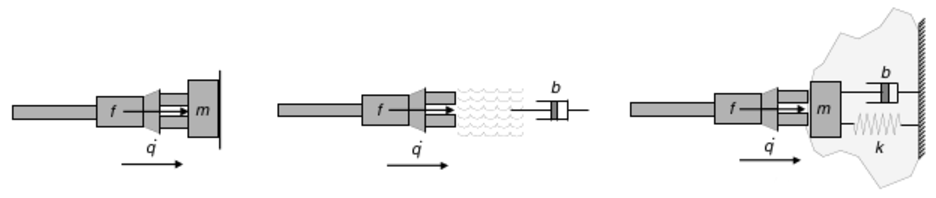
\includegraphics[scale=0.65]{type_of_impedances}
  \begin{itemize}
  \item[-] for each cartesian DoF the manipulator and the environment can be described using impedances $Z_m$ and $Z_e$
  \item[-] the environment is defined to be any element connected
    to or contacting the robot anywhere \alert{past the wrist} force sensor
  \item[-] $Z(\omega) = R(\omega) + j X(\omega)$
  \item[-] type of impedances
    \begin{itemize}
    \item[] inertial iff $|Z(0)| = 0$
    \item[] resistive iff $|Z(0)| = c \in (0, \infty)$
    \item[] capacitive iff $|Z(0)| \rightarrow \infty$
    \end{itemize}
  \end{itemize}
\end{frame}

\begin{frame}{HIC - Duality principle and equivalence to circuit theory}
  \begin{block}{Duality principle}
    The manipulator should be controlled to respond as the dual of the environment
  \end{block}

  This principle is most easily described in terms of Norton and Thèvenin equivalents
  \begin{itemize}
  \item[-] an inertial environment is represented using a Thèvenin equivalent
  \item[-] a capacitive environment is represented using a Norton equivalent
  \item[-] a resistive environment is represented using either a Thèvenin or a Norton equivalent
  \end{itemize}
\end{frame}

\begin{frame}{HIC - Duality principle for position control}
  Manipulator impedance chosen as the dual of the environment impedance in order to obtain zero
  steady state error to a step input
  \vskip0.1in
  \begin{columns}
    \begin{column}{0.5\columnwidth}
      \begin{flalign*}
        v = \frac{Z_m(s)}{Z_m(s) + Z_e(s)}v_{des} - \frac{F_{env}}{Z_e + Z_m}
      \end{flalign*}
    \end{column}
    \begin{column}{0.5\columnwidth}
      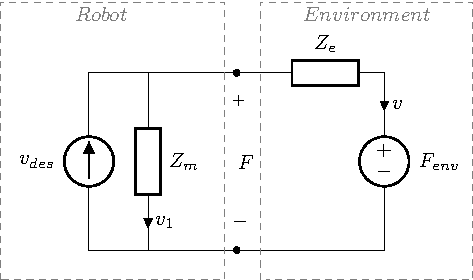
\includegraphics[width=\columnwidth]{position_control_model}
    \end{column}
  \end{columns}
  \[
  e_{ss} \Big|_{F_{env} \equiv 0} = \lim_{s \to 0}(v - v_{des}) = \frac{-Z_e(0)}{Z_m(0) + Z_e(0)} = 0 \text{ as long as } Z_m(0) \neq 0
  \]
  \begin{block}{Rule of thumb}
    inertial environments are position controlled with a noninertial manipulator impedances
  \end{block}
\end{frame}

\begin{frame}[shrink=30]{HIC - Position controlled subsystem}
  The electrical circuit can be seen as a control feedback scheme where $a$ is the ideal
  acceleration of the DoF corresponding to the desired velocity $v_{des}$
  \begin{columns}
    \begin{column}{0.4\textwidth}
      \begin{align*}
        &v_{des} = v + v_1\\
        &v_1 = \frac{F}{Z_m}\\ 
        &F = Z_e v + F_{env}\\
        &a = \dot{v} = \frac{\mathrm{d}}{\mathrm{d}t} \left(v_{des} - \frac{F}{Z_m} \right)\\
        &Z_m = M s + \tilde{Z}_m\\
      \end{align*}
    \end{column}
    \begin{column}{0.5\textwidth}
      \centering
      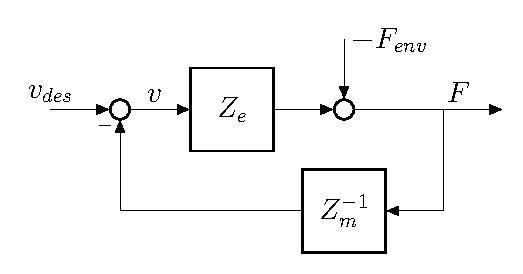
\includegraphics[scale=0.8]{position_control_feedback}
    \end{column}
  \end{columns}
  The acceleration can be written without derivatives
  \begin{align*}
    &a = \frac{\mathrm{d}}{\mathrm{d}t} \left(v_{des} - \frac{F}{Ms + \tilde{Z}_m} \right) = \dot{v}_{des} - \frac{Fs}{Ms + \tilde{Z}_{m}} = \dot{v}_{des} - s v_1 \\
    &F = v_1 (Ms + \tilde{Z}_m) \quad v_1 = \frac{F - (v_{des} - v)\tilde{Z}_m}{Ms}\\
    &a = \dot{v}_{des} - s v_1 = \dot{v}_{des} - \cancel{s} \left( \frac{F - (v_{des} - v)\tilde{Z}_m}{M\cancel{s}} \right) = \dot{v}_{des} + \frac{(v_{des} - v)\tilde{Z}_m}{M} - \frac{F}{M}
  \end{align*}
\end{frame}

\begin{frame}{HIC - Duality principle for force control}
  Manipulator impedance chosen as the dual of the environment impedance in order to obtain zero
  steady state error to a step input
  \vskip0.1in
  \begin{columns}
    \begin{column}{0.5\columnwidth}
      \begin{flalign*}
        F = \frac{Z_e(s)}{Z_m(s) + Z_e(s)}F_{des} + \frac{Z_e Z_m}{Z_m + Z_e} V_{env}
      \end{flalign*}
    \end{column}
    \begin{column}{0.45\columnwidth}
      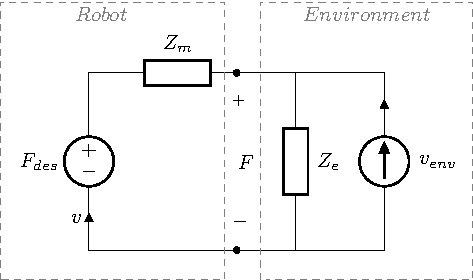
\includegraphics[width=\columnwidth]{force_control_model}
    \end{column}
  \end{columns}
  \[
  e_{ss} \Big|_{v_{env} \equiv 0} = \lim_{s \to 0}(F - F_{des}) = \frac{-Z_m(0)}{Z_m(0) + Z_e(0)} = 0 \text{ as long as } Z_m(0) < \infty
  \]
  \begin{block}{Rule of thumb}
    capacitive environments are force controlled with noncapacitive manipulator impedances
  \end{block}
\end{frame}

\begin{frame}[shrink=30]{HIC - Force controlled subsystem}
  The electrical circuit can be seen as a control feedback scheme where $a$ is the ideal
  acceleration of the DoF corresponding to the desired force $F_{des}$
  \begin{columns}
    \begin{column}{0.4\textwidth}
      \begin{align*}
        &F = F_{des} + Z_m v\\
        &v = \frac{F - F_{des}}{Z_m}\\
        &F = Z_e(v + v_{env})\\
        &a = \dot{v} = \frac{\mathrm{d}}{\mathrm{d}t} \left(\frac{F - F_{des}}{Z_m} \right)\\
        &Z_m = M s + \tilde{Z}_m\\
      \end{align*}
    \end{column}
    \begin{column}{0.5\textwidth}
      \centering
      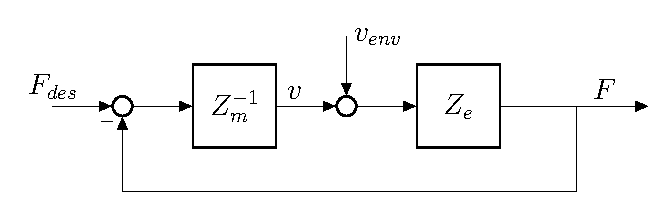
\includegraphics[scale=0.8]{force_control_feedback}
    \end{column}
  \end{columns}
  The acceleration can be written without derivatives
  \begin{align*}
    &a = \frac{\mathrm{d}}{\mathrm{d}t} \left(\frac{F - F_{des}}{Ms + \tilde{Z}_m} \right) = \left(\frac{s(F - F_{des})}{Ms + \tilde{Z}_m} \right)\\
    &vMs + v \tilde{Z}_m = F - F_{des}\\
    &v = \frac{1}{Ms} (F - F_{des} - v \tilde{Z}_m )\\
    &a = \dot{v} = \frac{\cancel{s}}{M\cancel{s}} (F - F_{des}) - \frac{\cancel{s}}{M\cancel{s}}( \tilde{Z}_m v) = \frac{1}{M} (F - F_{des}) - \frac{1}{M}( \tilde{Z}_m v)
  \end{align*}
\end{frame}

\section{HIC based control architecture}

\begin{frame}{References frames}
  Before delving into an HIC based controller let us introduce some useful reference frames and notation
  \begin{columns}
    \begin{column}{0.7\columnwidth}
      \begin{center}
        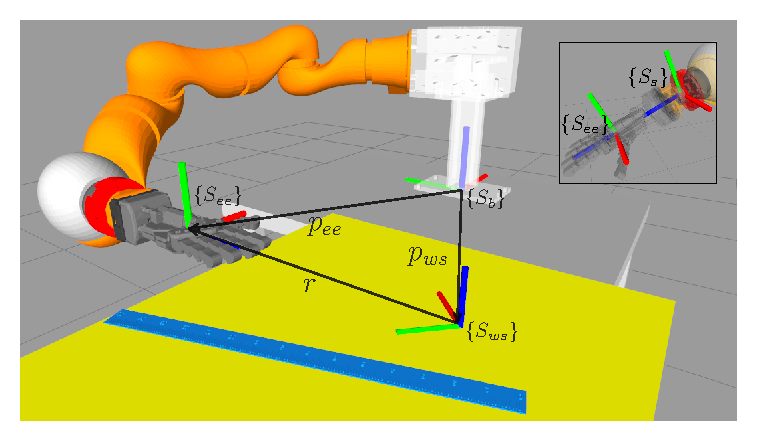
\includegraphics[width=\columnwidth]{frames_new}
      \end{center}
    \end{column}
    \begin{column}{0.3\columnwidth}
      \begin{itemize}
      \item[$b$:] base 
      \item[$s$:] sensor 
      \item[$ee$:] end-effector (hand) 
      \item[$ws$:] work-space (table) 
      \end{itemize}
    \end{column}
  \end{columns}
  \vskip-1em
  \begin{columns}
    \begin{column}{0.5\columnwidth}
      \begin{flalign*}
        &\{S_{b}\} = \{B; x_b, y_b, z_b \}\\
        &\{S_{s}\} = \{S; x_{s}, y_{s}, z_{s} \}
      \end{flalign*}
    \end{column}
    \begin{column}{0.5\columnwidth}
      \begin{flalign*}
        &\{S_{ee}\} = \{E; x_{ee}, y_{ee}, z_{ee} \}\\
        &\{S_{ws}\} = \{W; x_{ws}, y_{ws}, z_{ws} \}
      \end{flalign*}
    \end{column}
  \end{columns}
\end{frame}

\begin{frame}{Notation}
  \begin{block}{Space state vector definition}
    A natural choice for a basis in which the commanded positions and forces are expressed is $ws$
    \[
    \prescript{ws}{}{\vec{x}} = 
    \begin{bmatrix}
      \prescript{ws}{}{r}_x & \prescript{ws}{}{r}_y & \prescript{ws}{}{r}_z & \psi & \theta & \phi
    \end{bmatrix}^T
    \]
    \[
    \prescript{ws}{}{R}_{ee} = R_{ZYZ}(\psi, \theta, \phi) = R_{ZYZ}(\vec{\Phi})
    \]
  \end{block}
  \begin{block}{Convention}
    Convention used for any quantity $X$ encountered, $\prescript{b}{}{X}_p$
    \begin{itemize}
      \item[-] $\prescript{b}{}{.}$ reference frame
      \item[-] $._p$ reference point (for wrench and Jacobian only)
    \end{itemize}
  \end{block}
\end{frame}

\begin{frame}{Control aims}
  Suppose that the second derivative of the state can be chosen arbitrarily
  \[
  \prescript{ws}{}{\ddot{\vec{x}}} = \vec{a}_{cmd}
  \]
  Find $\vec{a}_{cmd}$ using HIC such that
  \begin{itemize}
  \item[-]$r_x$, $r_y$ and $\vec{\Phi}$ are rigidly controlled i.e.
    \begin{itemize}
    \item[i.] $\ddot{e}_{x} + B_x \dot{e}_x + K_x e_x = 0 \quad \quad  e_x(t) =   \prescript{ws}{} r_{x,des}(t) - \prescript{ws}{} r_{x}(t)$
    \item[ii.] $\ddot{e}_{y} + B_y \dot{e}_y + K_y e_y = 0 \quad \quad e_y(t) =   \prescript{ws}{} r_{y,des}(t) - \prescript{ws}{} r_{y}(t)$
    \item[iii.] $\ddot{\vec{e}}_{\Phi} + B_{\Phi} \dot{\vec{e}}_{\Phi} + K_{\Phi} \vec{e}_{\Phi} = \vec{0} \quad \quad \vec{e}_{\Phi}(t) = \vec{\Phi}_{des}(t) - \vec{\Phi}(t)$
    \end{itemize}
  \item[-]the DoF along $z_{ws}$ is force controlled i.e.
    \begin{itemize}
    \item[i.] $e_z \xrightarrow[t \to \infty] {} 0 \quad \quad e_{z}(t) = \prescript{ws}{} F_{z,des}(t) - \prescript{ws}{} F_{z}(t)$
    \end{itemize}
  \end{itemize}
  where $\prescript{ws}{} F_{z}(t)$ is the force exerted by the hand to the object expressed in $ws$
\end{frame}

\begin{frame}
  \frametitle{Hybrid Impedance control}
  \framesubtitle{Control assigned to each DoF}
  Position (${}^{ws}r_x,{}^{ws}r_y$):
  \begin{itemize}
  \item[-] inertial environment (manipulator moving a payload along given axis)
  \item[-] $Z_{m,p} = M_p s + \tilde{Z}_{m,p} = M_p s + B_p + \frac{K_p}{s}$
  \item[-] $a_{p} = a_{des,p} + \frac{B_p}{M_p} (v_{des,p} - v_p) + \frac{K_p}{M_p} (x_{des,p} - x_p) - \frac{F_p}{M_p}$
  \end{itemize}
  Attitude ($\psi$, $\theta$, $\phi$):
  \begin{itemize}
  \item[-] inertial environment (manipulator rotating a payload about given axis )
  \item[-] $Z_{m,a} = M_a s + \tilde{Z}_{m,a} = M_a s + B_a + \frac{K_a}{s}$
  \item[-] $a_a = a_{des,a} + \frac{B_a}{M_a} (v_{des,a} - v_a) + \frac{K_a}{M_a} (x_{des,a} - x_a)$
  \end{itemize}
  Force (${}^{ws}f_z$):
  \begin{itemize}
  \item[-] capacitive environment
  \item[-] $Z_{m,f} = M_f s + \tilde{Z}_{m,f} = M_f s + B_f$
  \item[-] $a_{f} = M_f^{-1}((f_{des} - f) - B_f v_z)$
  \end{itemize}  
\end{frame}

\begin{frame}
  \frametitle{Hybrid Impedance control}
  \framesubtitle{Filtering action}
  In principle one could assign a position control law \textcolor{red}{\emph{and}} a force
  control law for \textcolor{red}{\emph{each}} DoF
  
  A selection matrix $S$ is used to separate the force-controlled and position-controlled \emph{reciprocal} subspaces
  \begin{columns}
    \begin{column}{0.6\textwidth}
      \begin{flalign*}
        &\vec{a}_p = 
        \begin{bmatrix}
          a_{p,x} & a_{p,y} & a_{p,z}
        \end{bmatrix}^T&\\
        &\vec{a}_a = 
        \begin{bmatrix}
          a_{a, \psi} & a_{a, \theta} & a_{a, \phi}
        \end{bmatrix}^T&\\
        &\vec{a}_f = 
        \begin{bmatrix}
          a_{f,x} & a_{f,y} & a_{f,z} & a_{f, \psi} & a_{f, \theta} & a_{f, \phi}
        \end{bmatrix}^T&\\
        &\vec{a} = S 
        \begin{bmatrix}
          \vec{a}_p \\
          \vec{a}_a
        \end{bmatrix} + (I - S) \vec{a}_f&
      \end{flalign*}
    \end{column}
    \begin{column}{0.35\columnwidth}
      $
      S =
        \begin {bmatrix}
          1 & 0 & 0 & 0 & 0 & 0\\
          0 & 1 & 0 & 0 & 0 & 0\\
          0 & 0 & 0 & 0 & 0 & 0\\
          0 & 0 & 0 & 1 & 0 & 0\\
          0 & 0 & 0 & 0 & 1 & 0\\
          0 & 0 & 0 & 0 & 0 & 1\\
        \end {bmatrix}
      $
    \end{column}
  \end{columns}
\end{frame}

\begin{frame}
  \frametitle{Hybrid Impedance control}
  The resulting control law is
  \begin{align*}
    & a_x = \ddot{r}_{x,des} + B_x (\dot{r}_{x,des} - \dot{r}_x) + K_x (r_{x,des} - r_x) - F_x \\
    & a_y = \ddot{r}_{y,des} + B_y (\dot{r}_{y,des} - \dot{r}_y) + K_y (r_{y,des} - r_y) - F_y \\
    & a_z = - B_f \dot{r}_z + K_f(F_{z,des} - F_z) \\
    & a_{\psi} = \ddot{\psi}_{des} + B_{\psi}(\dot{\psi}_{des} - \dot{\psi}) + K_{\psi} (\psi_{des} - \psi) \\
    & a_{\theta} = \ddot{\theta}_{des} + B_{\theta}(\dot{\theta}_{des} - \dot{\theta}) + K_{\theta} (\theta_{des} - \theta) \\
    & a_{\phi} = \ddot{\phi}_{des} + B_{\phi}(\dot{\phi}_{des} - \dot{\phi}) + K_{\phi} (\phi_{des} - \phi) \\
  \end{align*}
\end{frame}
